\documentclass[12pt]{suhbook}
%% biber processes the reference db
%% citation keys and entries will be alphabetic
%% A reference section will be added to each chapter
\usepackage{amsmath}
\usepackage{commath}
\usepackage{mdwmath}
\usepackage{mathtools}
\usepackage{graphicx}
\usepackage{titlesec}
\usepackage{subcaption}
\usepackage{siunitx}
\sisetup{group-separator = {,}}
\usepackage[version=3]{mhchem}
% 
% 
% 
\begin{document}
% 
% 
% 
\setcounter{chapter}{3}% To jump to a chapter number, N-1 here
% 
% 
% 
\chapter{Flexible Terahertz Antenna Design for Wearable Applications}
% 
% 
% 
\section{Introduction}
% 
% 
Terahertz (THz) waves also known as sub-millimeter waves are observed between the optical and microwave frequency regions of the electromagnetic spectrum \cite{liu2009advanced,grischkowsky1990far}. Devices operating in the optical and infrared spectra are generally characterized by electromagnetic beams that contain many modes, and the dimensions of such devices is typically much larger than the operating wavelength. On the contrary, THz frequency based devices are comparable in size to the operating wavelength \cite{shi2018thz}. Such devices have the potential to fulfil the future wireless communications needs of ultra-high bandwidths and date rates. Moreover, the problems of channel congestion can be overcome through the use of THz based communication systems. 
There has been an ever increasing demand of the data-based wireless communication in the past decade. Moreover, throughout the world urban population has been growing at an alarming rate. These two factors have created enormous challenges in implementing high-speed and reliable networks that can serve a large number of people at the same time \cite{song2011present}. A natural solution to overcome this challenge is to shift the network operating frequency to the THz region. However, with the available technologies, THz systems are affected by high atmospheric attenuation, and therefore, much lower propagation distances. Hence, there is a demand for novel techniques through which the performance of a THz based communication system can be increased. To do so, micro and nano scale device fabrication techniques have actively been studied of late. Additionally, the search for highly conductive materials is an active research area to develop efficient THz devices.In conventional wireless communication systems, metallic antennas are fabricated separately from the microelectronics. It is not currently possible to operate circuitry in the THz frequency region simply by down-scaling the traditional metallic antenna to a few micrometres \cite{kleine2011review}. By moving up in the frequency, the device physics changes drastically and the approach of using a metal based antenna has several limitations, chief among them is the low mobility of electrons in the nano-scale metallic structures. This results in the antennas being highly lossy at the resonant frequencies, which would result in high attenuation and subsequently, poor efficiency of the overall system \cite{pourahmadazar2018millimeter}. To address this lossy behaviour, meta-material based nano-structures have emerged as attractive solutions \cite{chen2006active}.
Graphene is an atomically thin, two-dimensional crystalline form of carbon in which the carbon atoms are arranged in a hexagonal lattice structure. It was discovered in 2004 by Novoselov and Geim, who peeled off a small amount of monolayer graphene with the help of an adhesive tape, therefore, obtaining free-standing graphene in air \cite{novoselov2004electric}. For their ground-breaking discovery, they were awarded the Nobel Prize in Physics in 2010. Graphene is considered one of the thinnest yet in terms of mechanical properties, the strongest material measured  \cite{campos2008bulk,lee2013high}. Its theoretical specific surface area is as high as \SI{2630}{\square\m\per\gram}, thermal conductivity as high as \SI{5300}{\W \per \m \per \K}, which is higher than that of carbon nano-tube and diamond. In terms of electromagnetic properties, it is almost completely transparent, absorbing only \SI{2.3}{\percent} of light. On the other hand, graphene also has a very high electron mobility of \SI{15000}{\square \cm \per\V \per \siemens} at room temperature, which is higher than that of carbon nanotube or crystalline silicon \cite{ju2011graphene}. Nonetheless, the electrical resistivity of graphene is of the order of \SI{1e-6}{\ohm \cm} lower than copper and silver, which are the considered the best conducting materials. All these attractive characteristics enable graphene to display extra-ordinary electromagnetic phenomena. When an electromagnetic wave especially in the THz frequency range is obliquely incident wave upon graphene, surface plasmon polaritons (SPPs) are excited. Due to the high conductivity of graphene, the SPPs are tightly confined to the graphene surface having wavelength much smaller than its free-space equivalent. Moreover, the graphene SPPs exhibit moderate loss, and a vital property of tuning of the resonant frequency through external electrical and magnetic bias, and chemical doping. Most importantly, the resonant frequency of graphene lies in the THz and mid-infrared frequency ranges. Hence, this property, coupled with the lightweight and flexible nature of graphene open up the possibility of creating miniaturized and flexible antenna devices operating in the THz frequency domain that are well suited for wearable applications.

The electrical conductivity of graphene in the THz frequency range can be described using a semi-classical electronic model in the absence of magnetic bias. It is typically expressed in terms of the well-known frequency dependent Kubo formula, \cite{tamagnone2012analysis},
% 
\begin{equation} 
\sigma \left( \omega \right) \approx -j \frac{{e}^{2} k_{B} T}{\pi \hbar^{2}(\omega - j \tau^{-1})}  \times\left(\frac{\mu_{c}}{k_{B} T} + 2 \ln \left(e^{-\mu_{c} /\left(k_{B} T\right)}+1\right)\right) 
\label{eq:conductivity}
\end{equation}
% 
where $e$ is the electron charge, $\tau$ is the electron relaxation time in graphene, $k_B$ is the Boltzmann’s constant, $T$ is temperature, $\hbar$ is the reduced Planck’s constant, and $\mu_c$ is the chemical potential of graphene. The interband transitions (imaginary part in \eqref{eq:conductivity}) only occur when $\hbar \omega < 2\mu_c$, which is the case whilst operating in the THz frequency range for moderate $\mu_c$. For graphene, one of the most significant characteristics is the ability to control or in other words, tune the complex-valued conductivity. This can be done by exploiting the field effect field effect with an application of an external electrostatic field bias. The opto-electronic response of graphene can be described in terms of $\mu_c$ and $\tau$ as \cite{abadal2015time},
% 
\begin{subequations}
\begin{align}
    \mu_c ={}& \hbar v_f\sqrt{\pi N},
    \label{eq:chem_pot} \\
    \tau ={}& \frac{\mu_c \mu}{e v^2_f}
    \label{eq:rel_time}
\end{align}
\label{eq:opto}
\end{subequations}
% 
where $v_f$ is the Fermi velocity, $\mu$ is the carrier mobility of the electrons and $N$ is the carrier density. When $\mu_c$ and $N$ are low,  the complex-valued conductivity \eqref{eq:conductivity} has smaller real and imaginary parts. This leads to a poor efficiency in terms of radiation as the SPPs have a lower propagation length along the graphene surface. Therefore, in order to observe a strong resonant behaviour and improve efficiency, $\mu_c$ needs to be enhanced, which is usually done through chemical doping.Although both the increase in $\mu_c$ and $\mu$ lead to efficient radiation, the effect on the resonant frequency is different in both cases. Moreover, an increase in the radiated energy affects the width of the resonant frequency response introducing ringing tails around the center frequency. Such broadening of the temporal response is coherent with the sharpening of the resonant behaviour that is observed when the $\mu$ is increased. On the other hand, a stronger resonant behaviour is observed when $\tau$ is increased.
%
%
\\On ther other hand,  Perovskite is a sort of mineral that was first discovered in the Ural Mountains and named after a Russian scientist, Lev Perovskite  \cite{park2016organic}. A perovskite structure is any intensify that has a similar structure as the perovskite mineral. True perovskite (the mineral) is made out of calcium, titanium and oxygen in the structure \ce{CaTiO3}. Then, a perovskite structure is whatever has the conventional structure \ce{ABX3} and the equivalent crystallographic structure as the mineral perovskite \cite{chanana2017colour}. Perovskites have been widely inspected all around the world given their attractive properties especially regards to their photovoltaic and plasmonic applications \cite{song2015perovskite}. Perovskite materials display many outstanding characteristics in terms of superconductivity, ferro-electricity and high thermo-power \cite{kulkarni2012mixed}. Recently, there has been an increased interest in the leadhalide-based perovskite-type crystals owing to their extra-ordinary optical properties. They are self-organised low-dimensional crystals. However, \ce{CH3NH3PbI3} type perovskites have been recognized as promising materials, having a high carrier mobility, and diffusion length indicating that these materials can be to design antennas. Despite the attractive properties of perovskites, controlling the physical properties during the design and fabrication phased is still quite challenging, which is currently a limitation in the realization of next generation functional devices meant for high frequencies \cite{ahmad2017instability}. Moreover, various environmental factors including moisture, ultraviolet light exposure, and thermal stress play a key role in the instability of perovskite materials \cite{green2014emergence}.

\section{Graphene-based Antenna for Wearable Applications}
% 
A full-wave 3D electromagnetic simulation tool, CST Microwave Studio 2018 was used to analyze different antenna designs based on graphene acting as the main radiating element. All simulations were done at room temperature (\SI{293}{\kelvin}). In the first design, a patch antenna as shown in shown in Fig. \ref{Fig 1} was analyzed, which consisted of graphene as the conducting material, and a dielectric substrate. The effect of $\mu_c$ and $\tau$ on the radiation performance of the patch antenna was assessed by varying it in the range of \SI{0.1}{\eV} to \SI{0.4}{\eV},  \SI{0.1}{\ps} to \SI{0.8}{\ps}. The return loss of the patch antenna in the THz frequency range is shown in Fig. \ref{Fig 2}. It is noted that as $\tau$ is increased, the higher-order modes of the fundamental resonant frequency become prevalent.
% 
\begin{figure}[hbt!]
    \centering
    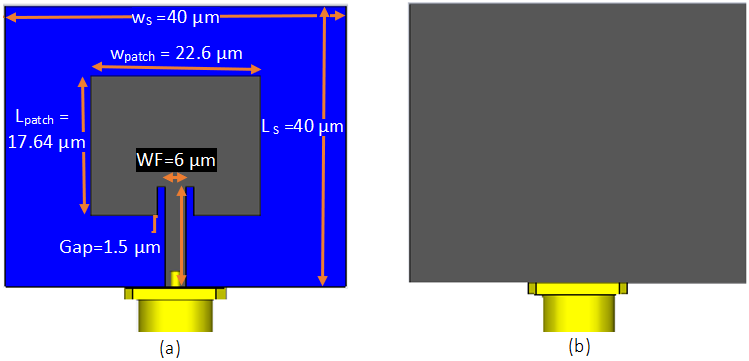
\includegraphics[width=0.52\textwidth]{1}
    \caption{Patch antenna with a flexible substrate and graphene as the radiating element.}
    \label{Fig 1}
\end{figure}
% 
\begin{figure}[h]
    \centering    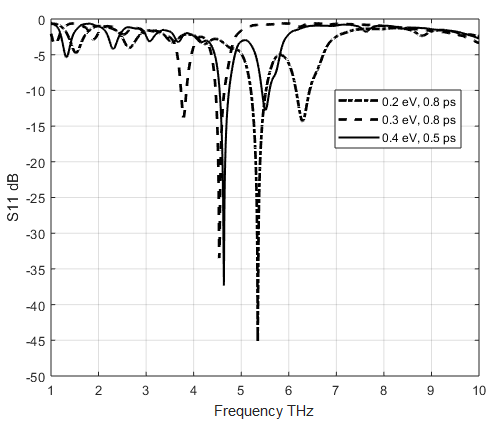
\includegraphics[width=0.5\textwidth]{2}
    \caption{The effect of chemical potential observed on the reflection coefficient ($\mathrm{S_{11}}$) in the THz frequency range. The value of $\mu_c$ was varied from, (black \SI{.2}{\eV}, blue \SI{.3}{\eV} to brown \SI{.4}{\eV}), whereas $\tau$ varied from \SI{.1}{\ps} to \SI{.5}{\ps}. }
    \label{Fig 2}
\end{figure}

The strongest resonance having the smallest value of ($\mathrm{S_{11}}$) is \SI{-45}{\dB} is obtained at at a chemical potential of \SI{0.4}{\eV} and \SI{0.5}{\ps} relaxation time. The resonant frequency of the graphene also changes when the chemical potential is varied. The effect is shown in Fig. \ref{Fig 2}. When $\mu_c$ has a value of \SI{0.4}{\eV}, the resonant frequency is observed at \SI{4.636}{\THz}, whereas at \SI{0.2}{\eV}, it is \SI{4.546}{\THz}. Furthermore,  the $\mathrm{S_{11}}$ started to increase from\SI{-34}{\dB} to almost \SI{-37}{\dB} . At \SI{0.4}{\eV}, $\mathrm{S_{11}}$ still below \SI{-10}{\dB} at \SI{0.1}{\ps } relaxation time, to get greater reflection coefficient, relaxation time must be increased, as result $\mathrm{S_{11}}$ increased to \SI{-45}{\dB} when relaxation time reaches \SI{0.5}{\ps }, the resonant frequency shifted to \SI{5.3}{\THz} as an alternative of \SI{4.7}{\THz} at \SI{0.3}{\eV}. The antenna has three possible resonant frequencies as shown in Table \ref{table:1}.The thickness of the substrate is evaluated to optimize the antenna performance in terms of the reflection coefficient and bandwidth. From Fig. \ref{Fig 3}, the substrate thickness obviously affects the $\mathrm{S_{11}}$ value, however, the bandwidth becomes narrower with increasing substrate thickness (Table \ref{table:2}).
% 
\begin{table}[hbt!]
\centering
 \begin{tabular}[hbt!]{|c | c |c |c|} 
 \hline
 $f$ (THz) & $\mu_c$ (eV) & $\tau$ (ps) & Bandwidth (GHz)\\ [0.5ex] 
 \hline
 4.546  & 0.2  & 0.8  & 185  \\ 
 \hline
 4.636  & 0.3  & 0.8  & 204  \\
 \hline
 5.347  & 0.4  & 0.5  & 310  \\
 \hline
\end{tabular}
\caption{The effect of chemical potential and relaxation time on resonant frequency and bandwidth.}
\label{table:1}
\end{table}
% 
% 
\begin{figure}[hbt!]
    \centering
    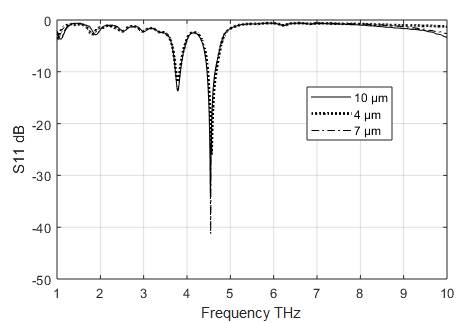
\includegraphics[width=0.5\textwidth]{3}
    \caption{Frequency sweep of the reflection coefficient for different values of substrate thickness.}
    \label{Fig 3}
\end{figure}
% 
% 
\begin{table}[hbt!]
\centering
 \begin{tabular}{|c |c |c |c|} 
 \hline
Substrate Thickness ($\mu m$) & f (GHz) & Bandwidth (GHz) &  $\mathrm{S_{11}}$ (dB) \\ [0.5ex] 
 \hline
4 & 4.546 & 193.9  & -26  \\ 
 \hline
7 & 4.546  & 192  & -41  \\
 \hline
 10 & 4.546  & 185  & -33.3 \\ 
 \hline
\end{tabular}
\caption{The effect of substrate thickness on the reflection coefficient and bandwidth.}
\label{table:2}
\end{table}
% 
As shown by the results, substrate thickness of \SI{7}{\um} generates the best resonance with $\mathrm{S_{11}}$ of \SI{-41}{\dB}, and a bandwidth of \SI{192}{\GHz}. The selection of substrate thickness is therefore a critical design parameter, which strongly affects the antenna resonance. For wearable electronic applications, a substrate material having flexibility is an essential requirement. In order to compare the performance of different types of flexible substrate materials, $\mu_c$ of \SI{0.2}{\eV}, and $\tau$ equal to \SI{0.8}{\ps} are selected. From Fig. \ref{Fig 4}, polyamide substrate (dielectric constant,$ \epsilon_r $= 4.5 and loss tangent, $\tan \alpha $= 0.0027) performs the best in terms of the $\mathrm{S_{11}}$ of \SI{-42}{\dB}. Polyamide substrate is appropriate for applications demanding a high degree of dimensional stability in extreme environmental conditions. Moreover, polyamide offers a high flexibility and low profile making it the perfect substrate material for printed fabrication techniques. On the other hand, Rogers 3006 substrate yielded a return loss of  \SI{-40.6}{\dB}, and for polyethylene terephthalate (PET), it was \SI{-30}{\dB}. For paper, the return loss was \SI{-30}{\dB}. 

The tunability of graphene is shown in Fig. \ref{Fig 5}, where the resonant frequency is changed with the help of chemical doping and applying an external voltage bias. Table \ref{table:3} provides a comparison of the three different resonant frequencies obtained for a substrate of thickness \SI{7}{\um}. All the frequencies have approximately the same $\mathrm{S_{11}}$ with the notable difference in bandwidth, which increases as the chemical potential increases. On the other hand, the transmission range gets lower when the electric potential is increased due to an increased absorption. In Figs. \ref{FIG 6} and \ref{FIG 7}, the radiation patterns illustrate high main lobe magnitudes along with lower back lobes levels. The main lobe magnitude in the E-plane starts from \SI{2.93}{\dB} at a chemical potential of \SI{0.2}{\eV}, and with increased $\mu_c$ the main lobe magnitude decreases to \SI{1.51}{\dB} at \SI{0.3}{\eV}, and \SI{-1.41}{\dB} at \SI{0.4}{\eV}.The proposed design suggests that the graphene-based patch antenna resonates at different frequencies in the THz band, \SI{4.546}{\THz}, \SI{4.636}{\THz} and \SI{5.347}{\THz} when the chemical potential and relaxation time are varied. Furthermore, changing the chemical potential leads to an increase in bandwidth from \SI{199}{\GHz} at\SI{0.2}{\eV} to \SI{314}{\GHz} at \SI{0.4}{\eV}. On the other hand, chemical potential affects the radiation pattern by increasing the side lobe and reducing the directivity of the proposed antenna. Analysis has also been performed to evaluate the antenna bandwidth and reflection coefficient ($\mathrm{S_{11}}$) at resonant frequencies. A comparison between different flexible substrates allows to evaluate the effect of substrate material on the antenna performance. A graphene-based antenna with polyamide substrate shows the maximum $\mathrm{S_{11}}$ of \SI{-42}{\dB}.
% 
\begin{figure}[hbt!]
\centering
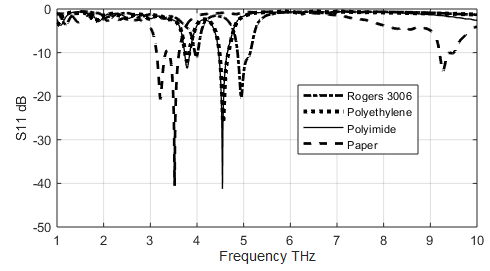
\includegraphics[width=0.51\textwidth]{4}
\caption{Reflection coefficient ($\mathrm{S_{11}}$) of different substrate material thickness \SI{7}{\um},  Rogers 3006,Polyethylene, Polyamide, Paper.}
\label{Fig 4}
\end{figure}
% 
\begin{figure}[h]
\centering
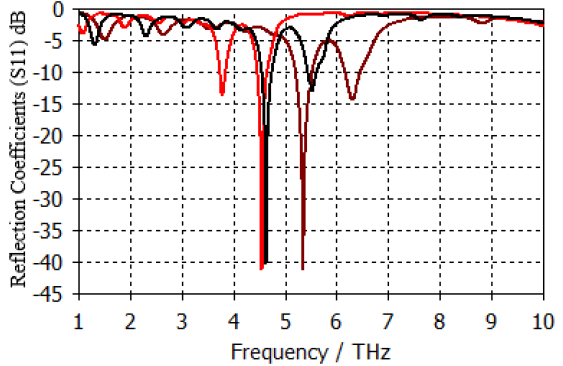
\includegraphics[width=0.5\textwidth]{5}
\caption{Antenna resonant frequencies at \SI{7}{\um} thickness (0.2 eV and 0.8 ps red, 0.3 eV and 0.8 ps, black 0.4 eV and 0.5 ps).}
\label{Fig 5}
\end{figure}
% 
\begin{table}[hbt!]
\centering
 \begin{tabular}[hbt!]{|c | c |c |c|c|} 
 \hline
 $f$ (THz) & $\mu_c$ (eV) & $\tau$ (ps) & Reflection Coefficient($\mathrm{S_{11}}$) & Bandwidth (GHz) \\ [0.5ex] 
 \hline
4.546 & 0.2  & 0.8  &  -41.258 & 199 \\
 \hline
4.636  & 0.3  & 0.8  & -40.187  & 279.9 \\
 \hline
 5.347 & 0.4  & 0.5 & -41.283 & 314  \\[1ex]
 \hline
\end{tabular}
\caption{A comparison between different resonant frequencies at \SI{7}{\um} substrate thickness.}
\label{table:3}
\end{table}
% 
% 
\begin{figure}[hbt!]
\begin{subfigure}{.5\textwidth}
  \centering
  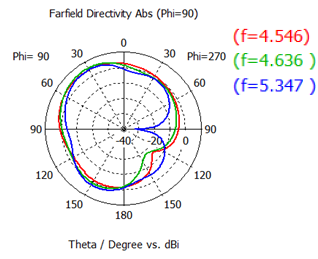
\includegraphics[width=.9\linewidth]{6}
  \caption{H-plane}
  \label{FIG 6}
\end{subfigure}%
\begin{subfigure}{.5\textwidth}
  \centering
  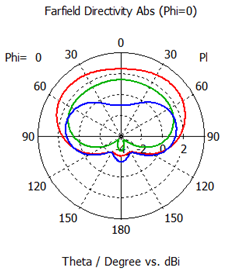
\includegraphics[width=.8\linewidth]{7}
  \caption{E-plane}
  \label{FIG 7}
\end{subfigure}
\caption{Simulations of the normalized field patterns in the E plane and H plane at different frequencies.}
\label{fig:fig}
\end{figure}
% 
% 
% 
\section{The Effect of Human Body on the antenna radiation characteristics}
% 
% 
The demand for wearable devices is expected to increase to \num{187.2}  million wearable units annually by \num{2022} \cite{hernandez2019wearable}. Wearable antenna requirements for all modern applications require lightweight, low-cost, and a flexible profile. For wireless body area network (WBAN) scenarios, the antenna design becomes more complicated than free-space environments, due to the absorption of the human skin. Human skin is a complex heterogeneous and anisotropic medium, where minuscule organs such as blood vessel and pigment content are spatially distributed in depth \cite{flynn2011modeling}. With the complexity of human skin, it is challenging to accurately describe the material, mainly due to the shapes and functions, and most importantly because of the absence of the dielectric constant measurements at high frequency \cite{alekseev2007human}. Therefore, most of the latest research simulates the human skin as three layers; epidermis, dermis, and hypodermis which represent the most essential parts of the human skin \cite{lynch1989growth}. Wearable antennas, therefore should be carefully designed to minimize skin absorption.
% 
\begin{figure}[hbt!]
\centering
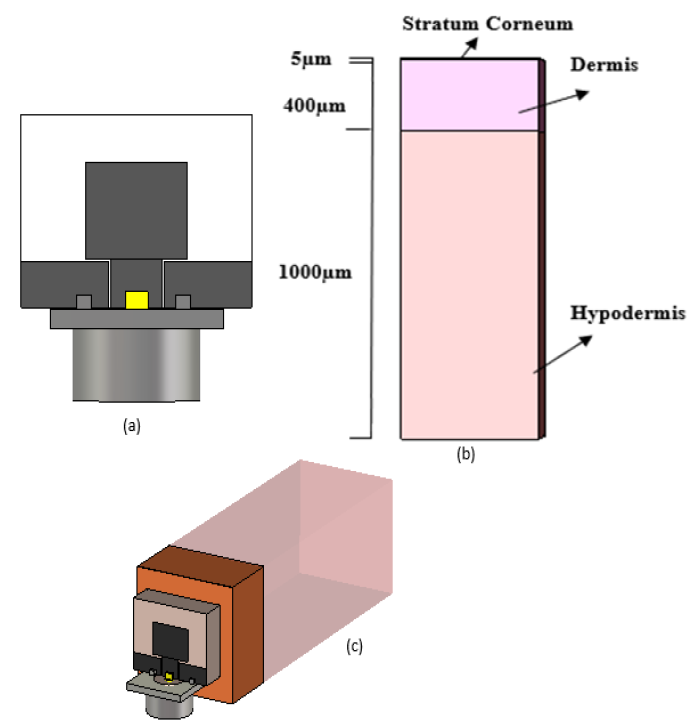
\includegraphics[width=0.6\textwidth]{8}
\caption{Geometry of the proposed patch antenna (a) Front view and (b) Human skin model (c) side view of the antenna on the human body.}
\label{Fig 8}
\end{figure}
% 
Figure \ref{Fig 8}a shows the geometry and parameters of the proposed co-planar waveguide (CPW) fed antenna. The antenna design is simulated in CST Microwave Studio 2018 at room temperature (\SI{293}{\kelvin}). The antenna design has the dimensions of \SI{260}{\um} by\SI{195}{\um} by \SI{0.35}{\nm}, with two layers of graphene, and consists of a graphene-based rectangular patch with a feedline \SI{120}{\um} by \SI{100}{\um} by \SI{0.35}{\nm} made from graphene. Rogers \num{3006}, having a dielectric constant of $\varepsilon_r = 6.5$, and loss tangent, $\tan {\alpha} = 0.002$ is used as substrate with a thickness of \SI{175}{\um}. Three layers of human skin model as shown in Fig. \ref{Fig 8}b, the thickness of which differ between various human skins. For the epidermis, the typical thickness ranges from  \SIrange{.05}{1.5}{\mm}, whereas the dermis is typically \SI{1.5e-4}{\mm}. The hypodermis, on the other hand has no typical value \cite{dashti2018graphene}. The epidermis is sibdivided into two further layers, stratum corneum with only dead squamous cells and the living epidermis layer, where most of the skin pigmentation stay \cite{abadal2015time}. The stratum corneum is a thin accumulation on the skin outer surface. The dermis, that supports the epidermis, is thicker and mainly composed of collagen fibers and intertwined elastic fibers enmeshed in a gel-like matrix. The subcutaneous fat layer is composed of the packed cells with considerable fat, where the boundary is not well defined, thus, the thickness of this layer differs widely for various part of the human body. The real ($\varepsilon^-$) and imaginary ($\varepsilon^=$) parts of the permittivity of the human skin tissues can be obtained using \cite{berry2003optical,yang2015numerical},
% 
\begin{subequations}
\begin{align}
   \varepsilon^- &= n^2-k^2,
   \label{eq:real perimttivity} \\
    \varepsilon^= &= 2nk
\label{eq:imag perimttivity}
\end{align}
\label{eq:permititivty}
\end{subequations}
% 
where  $n$ is the refractive index, and $k$ is the extinction coefficient. The refractive indices for blood, skin, and fat are \num{1.97}, \num{1.73} and \num{1.58} respectively \cite{yang2015numerical}. The extinction coefficient is calculated using the measured absorption coefficient data available in \cite{fitzgerald2003catalogue,berry2003optical} through,
% 
\begin{equation}
k=\frac{\alpha\lambda_0}{4\pi}
\label{eq:abdorption}
\end{equation}
% 
where $\lambda_0$ is the free-space wavelength, and $\alpha$ is the absorption coefficient. 

Figure \ref{Fig 8AE} demonstrates the scattering response of the graphene antenna in free-space. It is observed that resonant frequency can be downshifted with an increase in the patch length, in this case, from \SI{195}{\um} to\SI{215}{\um}. The $\mathrm{S_{11}}$ of the graphene patch antenna is \SI{-46}{\dB} at \SI{0.647}{\THz} obtained with length of \SI{195}{\um}. A wide  bandwidth of \SI{29.2}{\GHz} is also obtained which is an added advantage for wearable applications. Next, a comparison of antenna performance parameters is presented in a free-space environment and the on-body condition. From Fig. \ref{Fig 8B}, the reflection coefficient of the patch antenna in the on-body state is shifted slightly towards the right side of the \SI{0.6482}{\THz} resonant frequency.
% 
\begin{figure}[hbt!]
    \centering
    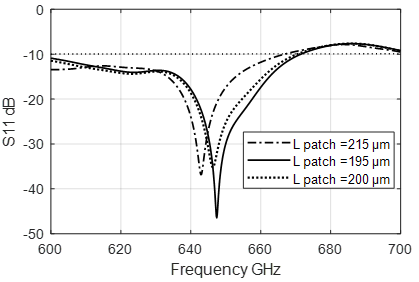
\includegraphics[width=0.6\textwidth]{9}
    \caption{$\mathrm{S_{11}}$ of the antenna with different patch lengths.}
    \label{Fig 8AE}
\end{figure}
% 
\begin{figure}[hbt!]
    \centering
    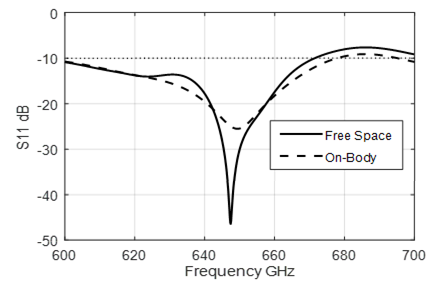
\includegraphics[width=0.6\textwidth]{10}
    \caption{$\mathrm{S_{11}}$ in the on-body and free-space conditions.}
    \label{Fig 8B}
\end{figure}
% 
\begin{figure}[hbt!]
    \centering
    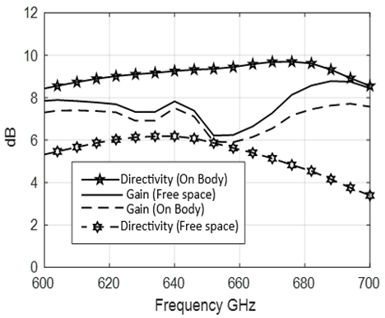
\includegraphics[width=0.6\textwidth]{11}
    \caption{Simulation gain and directivity in free-space and on-body conditions.}
    \label{Fig 8AA}
\end{figure}
% 
\begin{figure}[hbt!]
    \centering
    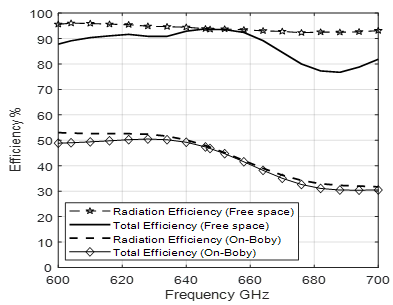
\includegraphics[width=0.47\textwidth]{12}
    \caption{Radiation and total efficiencies in free-space and on-body conditions.}
    \label{Fig 91}
\end{figure}
% 
\begin{figure}[hbt!]
\begin{subfigure}{.4\textwidth}
\centering
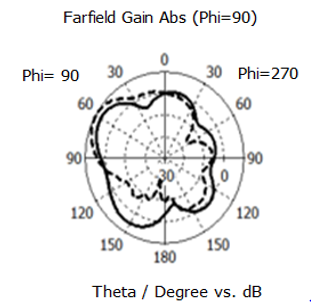
\includegraphics[width=.9\linewidth]{13}
\caption{H plane}
\label{fig:sfig10a}
\end{subfigure}%
\begin{subfigure}{.4\textwidth}
  \centering
  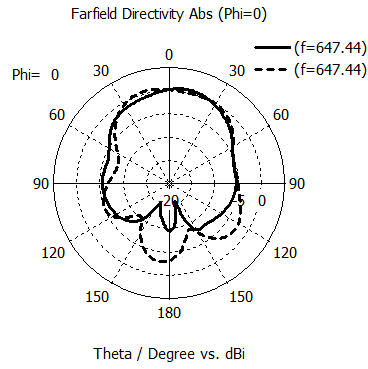
\includegraphics[width=.9\linewidth]{14}
  \caption{E plane}
  \label{fig:sfig2}
\end{subfigure}
\caption{The H- and E-plane radiation patterns of the graphene patch antenna in the on-body and free-space conditions.}
\label{fig 14b}
\end{figure}
% 
The $\mathrm{S_{11}}$ of the graphene patch antenna for the on-body case is \SI{-25}{\dB}. The shift in frequency is due to the high dielectric constant property of three layers of the human body in proximity with the antenna. Because of these properties of the human body, most of the radiated waves propagate through the body and dissipate in the form of heat resulting in a wider \SI{-10}{\dB} bandwidth. Due to the body absorption, the antenna gain decreases from \SI{-7.8}{\dB} to \SI{-7.2}{\dB}. The antenna gain is a figure of merit of how well the antenna converts the power supplied into radiated waves in a specific direction. For the case of the on-body condition, a lower value of the gain is obtained which is due to a decrease in the radiation efficiency, down from \SI{96}{\percent} to almost \SI{50}{\percent} (Fig. \ref{Fig 91}). Therefore, the total radiated efficiency of antenna on a flat body phantom decreases by nearly a factor of two. This is due to the higher conductivity of the outer most layer skin. The antenna total efficiency in the presence of the human body also decreases due to absorption in the lossy human body tissues. The H- and E- plane radiation patterns of the graphene patch antenna in the on-body and free-space conditions are shown in Fig. \ref{fig 14b}. The main lobe with \SI{-6.87}{\dB} is obtained at the resonance of \SI{0.647}{\THz}, while an increase in the magnitude of the main lobe is observed at on-body state with \SI{9.7}{\dB}. Similarly, the side lobe in the on-body case is \SI{-8}{\dB} and on free-space is \SI{-2}{\dB}  due to higher reflections from the body surface.
A wearable graphene THz antenna is presented and tested on three layers of human skin to serve the wearable applications in modern THz systems to achieve high performance. The results show that the designed antenna presented at \SI{0.647}{\THz}, has a realized gain of \SI{7.8}{\dB} and \SI{7.2}{\dB} in the free-space and on-body cases respectively. The radiation efficiency dropped from \SI{96}{\percent} to \SI{50}{\percent} when placed on the body.
\section{Perovskite-based Antennas}
% 
 With the increasing demands of high speed, reliable and secure wireless communication and safety of the user in terms of radiation exposure, research trends have shown a migration towards high-frequency THz spectrum \cite{ghann2017terahertz,rabbani2017liquid}. Recent research efforts have been focused to overcome the propagation and fabrication issues at THz and in developing THz sources, antennas, systems and applications \cite{siegel2002terahertz}. Therefore, THz devices can now be found in applications such as bio-sensing and imaging, fast and secure wireless systems, and radar communication \cite{ranzani2013g,khatib2018response}. Due to high absorption levels of THz waves by the water molecules and limited penetration ability into the human body, the probability to produce hazardous ionization of biological tissues is low, which is an advantage of current medical imaging techniques such as x-rays. An efficient antenna is critical in developing a high-performance THz system. Therefore, several design aspects need to be considered to develop an antenna which is able to fulfill the demands of THz applications \cite{chen2016research}. Rapid progress has been made in the utilization of low-dimensional materials moving on from traditional copper-based radiating patch, which generate high loss and poor efficiency due to decrease in skin depth and conductivity in the THz frequency band. Carbon-based materials i.e. graphene, and carbon nano-tubes have shown promise in this regard \cite{naghdehforushha2017design}. Perovskites, due to the features such as superconductivity, ferro-electricity and low cost, have gained focus in various novel applications \cite{huang2014low}.The proposed antenna design is numerically analysed using CST Microwave Studio at room temperature (\SI{293}{\kelvin}). Perovskite material is simulated using the measured permittivity values as described in \cite{green2014emergence}. Figure \ref{fig:fig 11b} shows the antenna design with the dimensions \SI{40}{\um} by \SI{40}{\um} by \SI{10}{\um}, consisting of a perovskite based rectangular patch, while the ground plane and feedline are made of copper. Thin flexible film of polyamide is used as a substrate.
% 
\begin{figure}[hbt!]
\begin{subfigure}{.5\textwidth}
\centering
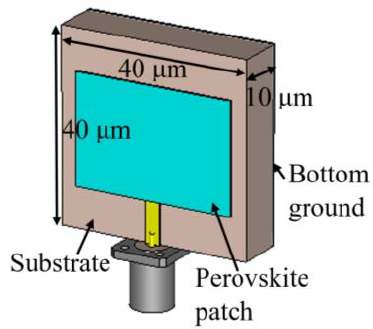
\includegraphics[width=.9\linewidth]{15}
\caption{simulated antenna design;}
\label{fig:sfig11a}
\end{subfigure}%
\begin{subfigure}{.4\textwidth}
  \centering
  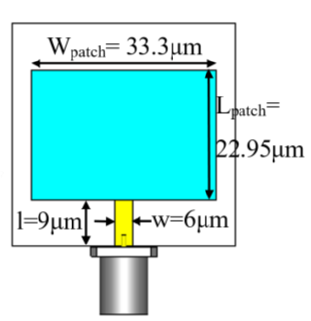
\includegraphics[width=.9\linewidth]{16}
  \caption{perovskite patch and copper feed line in the antenna prototype.}
  \label{fig:sfigb11}
\end{subfigure}
\caption{Proposed perovskite-based THz antenna.}
\label{fig:fig 11b}
\end{figure}
% 
A frequency sweep of the reflection coefficient of the perovskite-based antenna is shown in Fig. \ref{Fig 17}, which demonstrates two significant bands while taking \SI{-10}{\dB} as a reference. The first band lies in the range \SIrange{3.6}{7.4}{\THz} and constitutes two dominant resonances at \SI{5.18}{\THz} and \SI{6.98}{\THz}. The second band covers \SIrange{8.25}{10}{\THz} with a notable resonant dip at \SI{8.8}{\THz}. A parametric analysis is carried out on the radiating length of the antenna, the results of which are shown in Fig. \ref{Fig 18}. It is observed that with the increase in length from \SI{20.95}{\um} to \SI{29.7}{\um}, the resonant frequency is shifted down. The gain and efficiency versus frequency plots are shown in Fig. \ref{Fig 119}, which indicate that the realized gain varies from \SI{-4.8}{\dB} in the overall operating range. The gain magnitude is above \SI{4}{\dB} throughout the frequency sweep. Simulated results as shown in Fig. \ref{Fig 119} also present good efficiency of \SI{88}{\percent} at \SI{5.185}{\THz}, which is comparable to the reported graphene-based THz antenna in \cite{dashti2018graphene}. In addition, the radiation efficiency of the designed antenna can further be improved by increasing the conductivity of perovskite film with the application of an external voltage.
% 
\begin{figure}[hbt!]
\centering
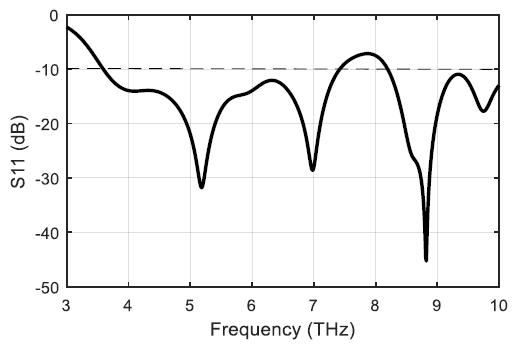
\includegraphics[width=0.5\textwidth]{17}
\caption{Simulated $\mathrm{S_{11}}$ profile of the designed perovskite-based THz antenna.}
\label{Fig 17}
\end{figure}
\begin{figure}[hbt!]
\centering
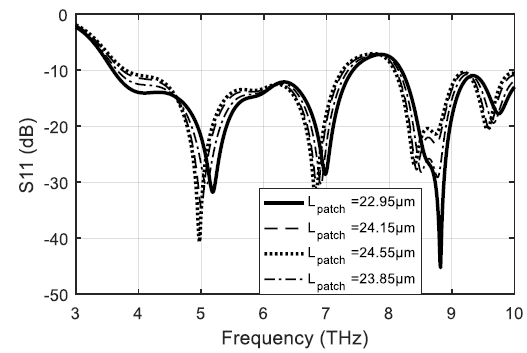
\includegraphics[width=0.5\textwidth]{18}
\caption{Parametric analysis of the radiating length of the designed perovskite based THz antenna.}
\label{Fig 18}
\end{figure}
\begin{figure}[hbt!]
\centering
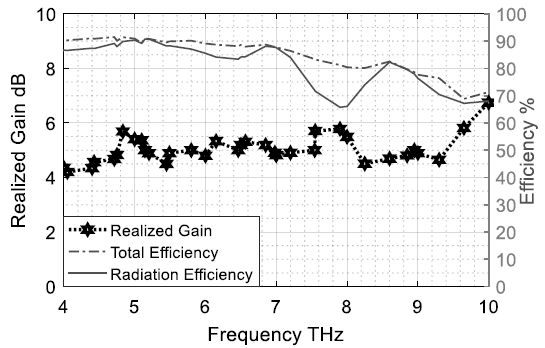
\includegraphics[width=0.5\textwidth]{19}
\caption{Realized gain and efficiency plots of the proposed perovskite based THz antenna.}
\label{Fig 119}
\end{figure}
% 
The E- and H-plane radiation patterns of the designed antenna at the three major resonant frequencies are illustrated in Fig. \ref{fig:fig 15}. The main lobe with \SI{4.53}{\dB} is obtained at the resonance of \SI{5.185}{\THz}, while an increase in the magnitude of the main lobe gain is observed at \SI{6.985}{\THz} and \SI{8.821}{\THz} resonances. Although the radiation is not perfect broadside in the complete operating range, this effect is obvious when the antenna is designed to cover a wide bandwidth. The high bandwidth, reasonable gain magnitudes and high efficiency depict that the perovskite can be deployed as a radiating element in the THz patch antennas.
% 
\begin{figure}[hbt!]
\begin{subfigure}{.45\textwidth}
\centering
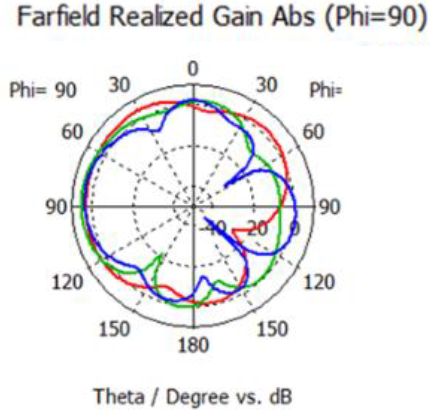
\includegraphics[width=0.9\linewidth]{20}
\caption{E-Plane}
\label{fig:sfig15a}
\end{subfigure}%
\begin{subfigure}{.45\textwidth}
  \centering
  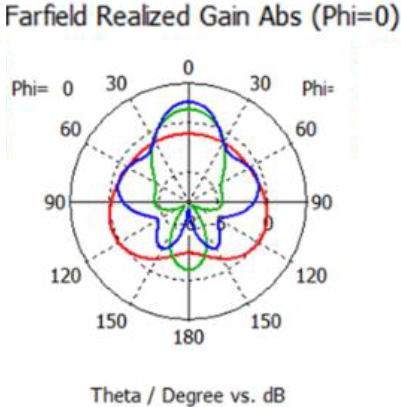
\includegraphics[width=0.9\linewidth]{21}
  \caption{H-Plane}
  \label{fig:sfigb15}
\end{subfigure}
\caption{Proposed perovskite-based THz antenna.}
\label{fig:fig 15}
\end{figure}
% 
The THz antennas are anticipated to ensure a high resolution imagining for the biomedical applications due to their short wavelength and high directivity. Novel materials have been developed for the potential deployment in modern THz systems to achieve high performance.  A newly developed perovskite material has been used for the antenna design which can replace the conventional metallic patches. The results show that the designed antenna covers two THz bands, \SIrange{3.6}{7.4}{\THz} and \SIrange{8.25}{10}{\THz}. The realized gain of the antenna is above \SI{4}{\dB} and radiation efficiency is above \SI{70}{\percent} in overall operating bandwidth. The antenna is regarded as a potential candidate for the future short-range THz communications.

\section{Conclusion}
In this chapter, an overview of wearable antennas operating in the terahertz frequency range, and made from two-dimensional materials such as graphene is presented. The antenna designs are analyzed in realistic environments in the proximity of human skin. Characteristics such as highly miniaturized and flexible substrate materials of the antennas coupled with excellent antenna performance make these wearable antennas a strong candidate in applications of short-range wireless communication near human body. The resonant properties of the two-dimensional materials are investigated using their electronic properties.  Wireless communication in the terahertz frequency, high-resolution imaging for biosensing and disease management, and spectroscopy are anticipated to be some of the early beneficiaries of wearable and flexible antennas. Further investigations in this area of research provide interesting opportunities not only for the antenna engineers, but material scientists and physicists as well.
% 
% 
\bibliography{bibliography.bib}
\bibliographystyle{unsrt}
\end{document}